\chapter{Arbetet}
Arbetet kan del


Stort problem är att json och json scheman inte skiljer på heltal och reela tal, medan många språk gör det. Specifikt Delphi som systemet utvecklades i.

Ingen har beskrivit parsning av JSON Schema!!!

\section{Systemet i helhet}

När administrationsprogrammet kopplar upp sig mot servern skickar servern ett JSON Schema, tillsammans med en JSON-fil som beskriver den riktiga datan. Det flödet illustreras i figur \ref{fig:system:ner}. Hur datan sedan propageras upp från användargränssnittet, till servern illustreras i figur \ref{fig:system:upp}.

\begin{figure}
	\begin{subfigure}[b]{0.5\textwidth}
		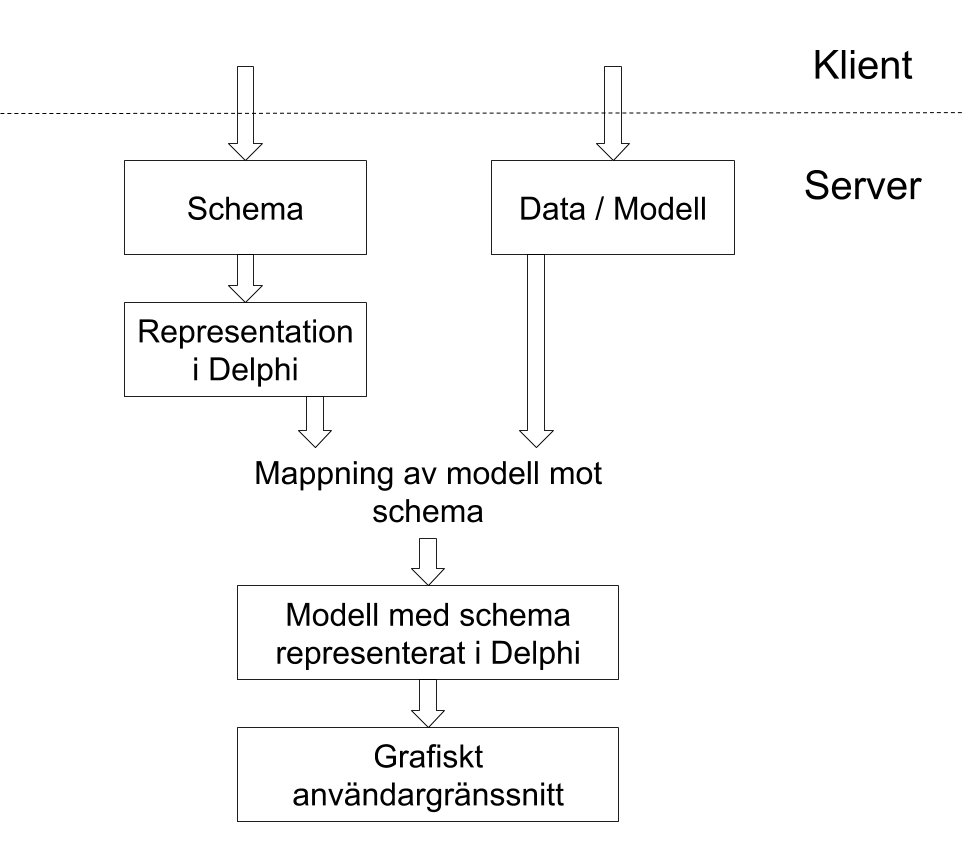
\includegraphics[width=0.9\textwidth,left]{./img.png}
		\caption{Flödesschema över systemet}
		\label{fig:system:ner}
	\end{subfigure}
	\begin{subfigure}[b]{0.5\textwidth}
		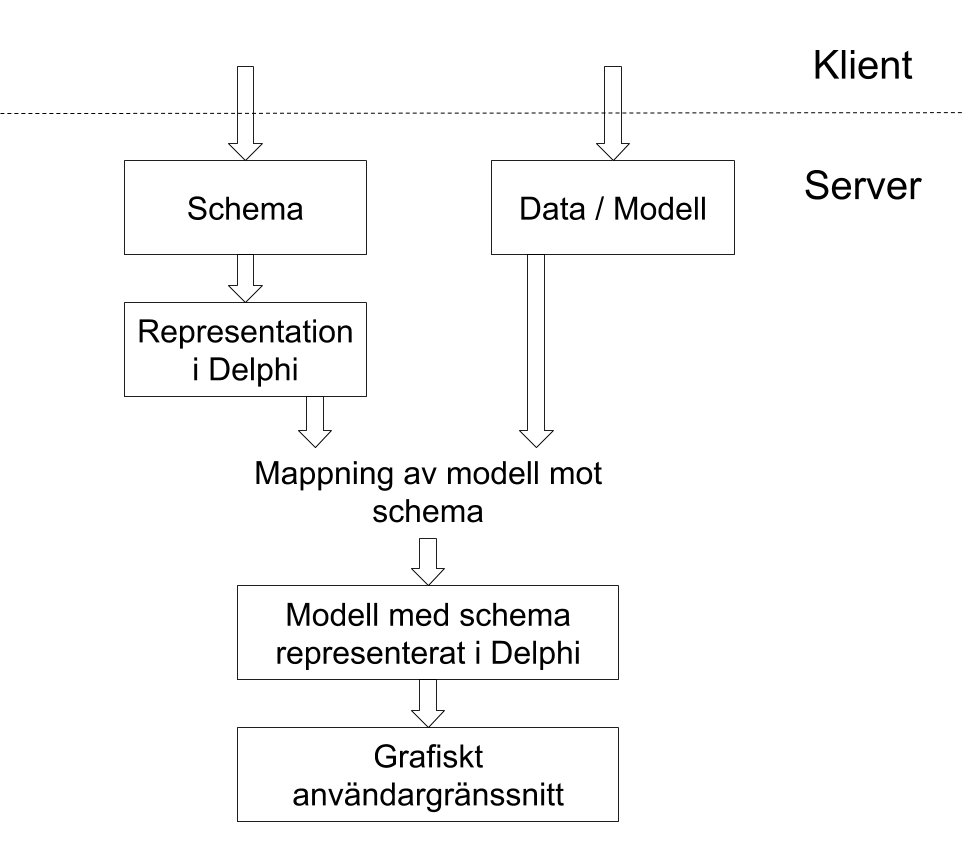
\includegraphics[width=0.9\textwidth,right]{./img.png}
		\caption{Flödesschema över systemet}
		\label{fig:system:upp}	
	\end{subfigure}
	\caption{Illustration av dataflöde till och från användargränssnittet}
	\label{fig:system}
\end{figure}

\section{Generering av JSON Schema i Delphi}


\section{Parsningen av JSON Schema i Delphi}


\section{Representation av data i användargänssnittet}


\section{Manipulering av data utifrån användarinteraktion}
